\documentclass[12pt]{article}
\setlength{\columnsep}{0.8cm}
\usepackage{fullpage}
\usepackage{graphicx,graphics}
\usepackage{mathtools}
\usepackage{subcaption}
\usepackage{multirow}
\usepackage{multicol}
\usepackage{listings}
\DeclarePairedDelimiter\ceil{\lceil}{\rceil}
\DeclarePairedDelimiter\floor{\lfloor}{\rfloor}

\begin{document}
	
\noindent\centerline{\LARGE{College Football Bowl Game Predictions}}
\noindent\centerline{}
\noindent\centerline{}
\noindent\centerline{Spring 2015}
\noindent\centerline{15.077 Final Project}
\noindent\centerline{Geoffrey Gunow}
%\maketitle

\section{Introduction}
College Football has grown to be one of the most popular competitive sports over the last few decades. Indeed, sports betting on college football is a multi-billion dollar industry. In addition, many organizations such as ESPN offer cash prize competitions for predicting outcomes of games. In particular, ESPN is renowned for it's College Football Bowl Pick 'em Challenge. In this game, each player attempts to predict the winner of all $N$ college football bowl games. In addition, the player assigns confidence points ranging from 1 to $N$ on each game with no repeated numbers. If the player correctly predicts the outcome, they receive the confidence points assigned to the game. If they incorrectly predict the outcome, they receive no points. The player with the highest point total at the end of the games wins. Therefore to maximize the point total, the player should assign the highest confidence points to games in which the player is very certain of the outcome, and the lowest points to uncertain outcomes.

In this project, I concentrate on being able to accurately predict the outcomes of bowl games and also form a measure of confidence for each prediction. Therefore, multiple models are developed for predicting the outcomes of bowl games and methods for deriving confidence measures are discussed. Throughout this project, I make heavy use of the python package Scikit-learn \cite{scikit-learn}. All methods and analysis used in this report are based on Scikit-learn or self-implemented software.

\section{Data Scraping and Feature Formation}
First data needs to be gathered on each team participating in a bowl game in order to form features. This data is formed from regular season statistics. \textit{Sunshine Forecast Downloadable Data Files} \cite{sunshine} provides data for each Division I FBS football game played from 2002 through 2013 in CSV format, a total of 383 bowl games. This data is scraped to produce easily-accessible dictionaries for the formation of features. Attributes provided for each team in this data are listed in Fig.~\ref{fig::attributes}.
\begin{figure}[ht!]
	\fbox{\parbox{\textwidth}{
	\begin{multicols}{3}
		\begin{itemize}
			\scriptsize
			\item Offensive Pass Completions
			\item Offensive Pass Attempts
			\item Offensive Pass Interceptions
			\item Offensive Pass Yards
			\item Offensive Rush Attempts
			\item Offensive Rush Yards
			\item Offensive Fumbles
			\item Defensive Pass Completions
			\item Defensive Pass Attempts
			\item Defensive Pass Interceptions
			\item Defensive Pass Yards
			\item Defensive Rush Attempts
			\item Defensive Rush Yards
			\item Defensive Fumbles
			\item Points For
			\item Points Against
			\item Games Played
			\item Wins
			\item Losses
			\item Winning Percentage
		\end{itemize}
	\end{multicols}}}
	\caption{Attributes for each team provided by \textit{Sunshine Forecast Downloadable Data Files}.}
	\label{fig::attributes}
\end{figure}

In addition to these 21 attributes, the number of takeaways, giveaways, and turnover margin are calculated from these statistics leading to a total of 24 attributes. For each attribute, a feature for the game averaged value is created when applicable (games played, wins, and losses are not normalized by the number of games). An additional 24 features are created for games just against teams playing in bowl games. The idea behind creating these features is to factor in how teams perform against strong teams. With these features added, information about the strength of schedule is implicitly added. These 48 features are formed for both teams. Finally, the Vegas betting line is added, leading to a total of 97 features. Each game is categorized in terms of whether the home team won the game. With such a large number of features relative to the size of the dataset, regularization is very important. Data is partitioned into train, validate, and test sets based on a 50\%, 30\%, and 20\% split respectively.

\section{Feature Analysis}
Now that the feature set is formed, it is often instructive to look at the data to get a sense of the underlying trends. First, we look at the normality of the features. Some algorithms rely on the assumption that the data is normally distributed. For instance, the Naive Bayes approach assumes that within each class the underlying features are normally distributed. To test this assumption, histograms are first created for every feature. For the purpose of illustration, the distribution of two features: the home team offensive rush yards per game and the visiting team defensive rush yards per game are plotted in Fig.~\ref{fig::features_hist}.

\begin{figure}[ht!]
	\centering
	\begin{subfigure}{.5\textwidth}
		\centering
		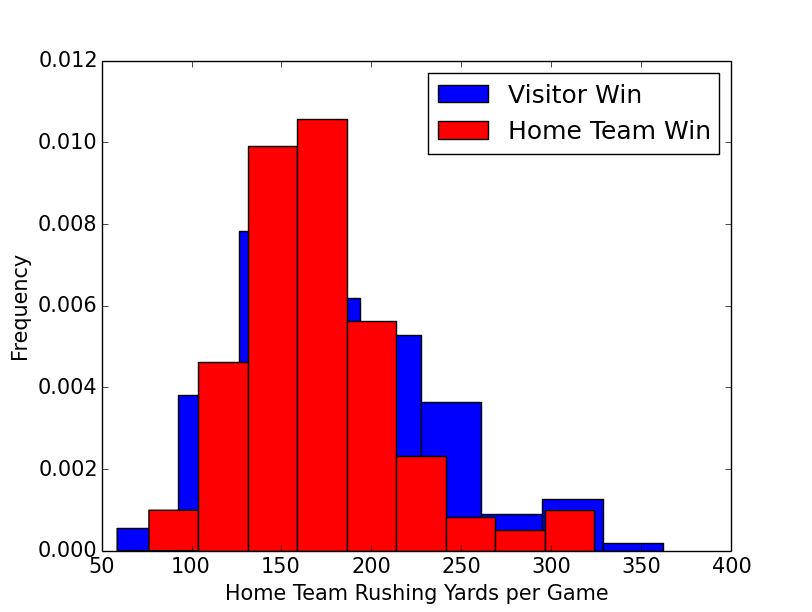
\includegraphics[width=.9\linewidth]{figs/homeRushOff.png}
		\caption{Home Team Rushing Offense}
		\label{fig::homeRushOff}
	\end{subfigure}%
	\begin{subfigure}{.5\textwidth}
		\centering
		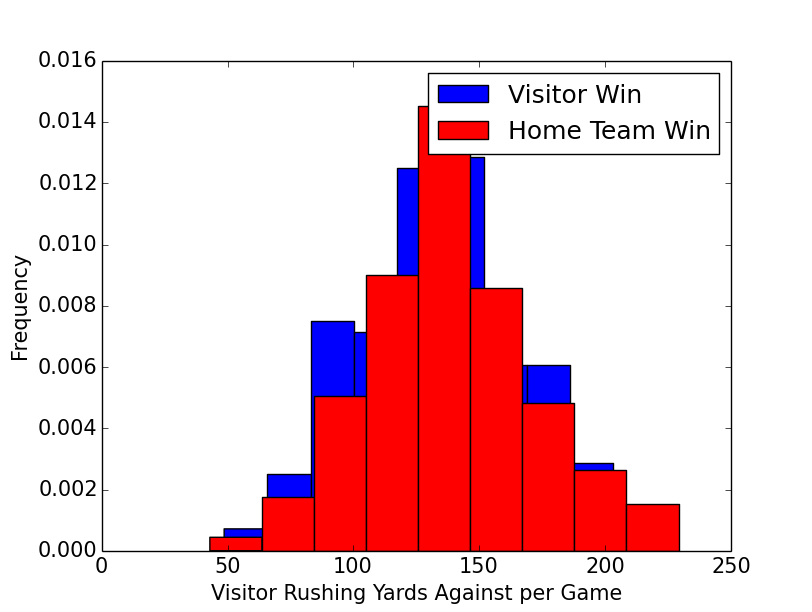
\includegraphics[width=.9\linewidth]{figs/visitorRushDef.png}
		\caption{Visitor Rushing Defense}
		\label{fig::visitorRushDef}
	\end{subfigure}
	\caption{Observed distributions of home team offensive rushing yards per game and visitor defensive rushing yards against per game.}
	\label{fig::features_hist}
\end{figure}

We see for home team wins, the average visitor rushing yards against per game seems to follow a normal distribution well, but the home team rushing yards per game seems to have a skew. Normality can be better viewed using a quantile-quantile plot. For a truly normal distribution, the quantile-quantile plot should show a straight line. Deviations from a straight line might indicate a skew in the data. The quantile-quantile plot for these two features is shown in Fig.~\ref{fig::QQ}.

\begin{figure}[ht!]
	\centering
	\begin{subfigure}{.5\textwidth}
		\centering
		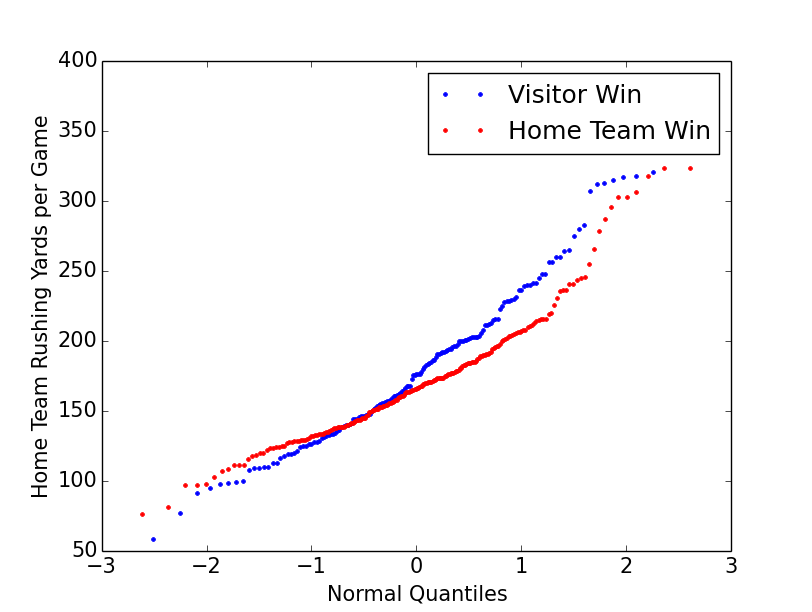
\includegraphics[width=.9\linewidth]{figs/homeRushOff_norm.png}
		\caption{Home Team Rushing Offense}
		\label{fig::homeRushOff_qq}
	\end{subfigure}%
	\begin{subfigure}{.5\textwidth}
		\centering
		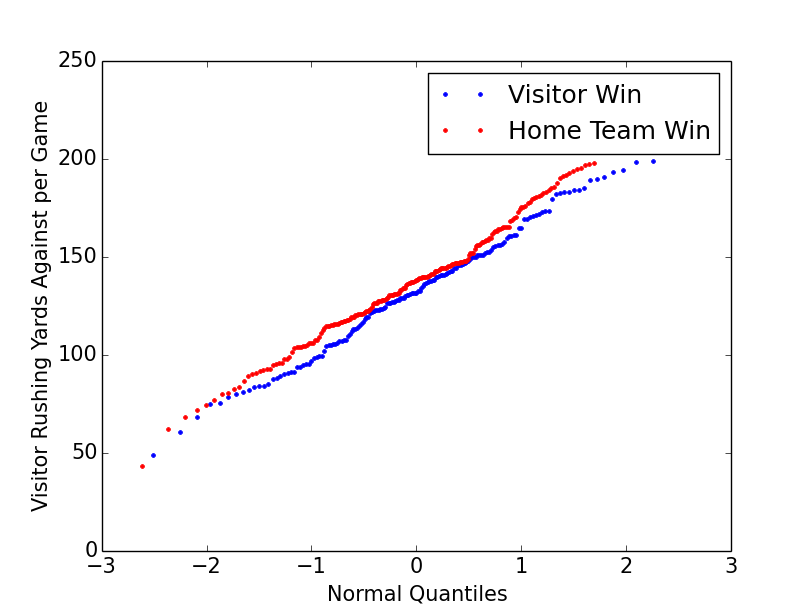
\includegraphics[width=.9\linewidth]{figs/visitorRushDef_norm.png}
		\caption{Visitor Rushing Defense}
		\label{fig::visitorRushDef_qq}
	\end{subfigure}
	\caption{Normal quantiles for home team offensive rushing yards per game and visitor defensive rushing yards against per game.}
	\label{fig::QQ}
\end{figure}

Note that the visitor rushing defense is quite linear on the quantile-quantile plot, suggesting that the normality assumption might be reasonable. However for the home team rushing offense, we see that at large values the quantile-quantile curve is highly non-linear, which is a manifestation of the skew observed from simply looking at the histogram. It might be possible to apply a transform to the data to eliminate the non-normality. Indeed, when a logarithmic transformation is applied to the home team rushing offense, the quantile-quantile plot becomes far more linear. However, transformations did not seem to impact the results greatly as many of the methods do not require the normality assumption. Therefore, the remaining results presented here will use non-transformed data.

Finally, to understand the interaction between these two chosen features, we plot them together in Fig.~\ref{fig::separation}.
\begin{figure}[ht!]
	\begin{center}
		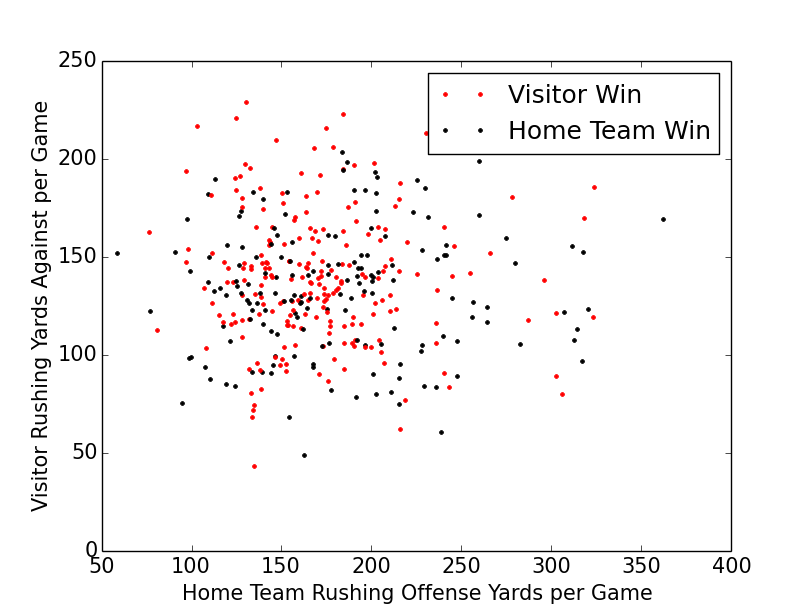
\includegraphics[scale=0.45]{figs/rush_matchup.png}
	\end{center}
	\caption{Bowl game results plotted against home team rushing offense and visitor rushing defense.}
	\label{fig::separation}
\end{figure}
Notice that the data does not seem to be very separable. Similar results are observed for all pairs of features in the data set. This hints that correctly classifying bowl game results might be a difficult task. 
\newpage
Perhaps a more accurate view of this data can be determined using principal component analysis (PCA) which applies a singular value decomposition to the feature data and returns the most significant singular vectors. These singular vectors can be a composition of any number of features. The two most significant features are shown in Fig.~\ref{fig::pca}. We see once again that there is no obvious separation in the data.
\begin{figure}[h!]
	\begin{center}
		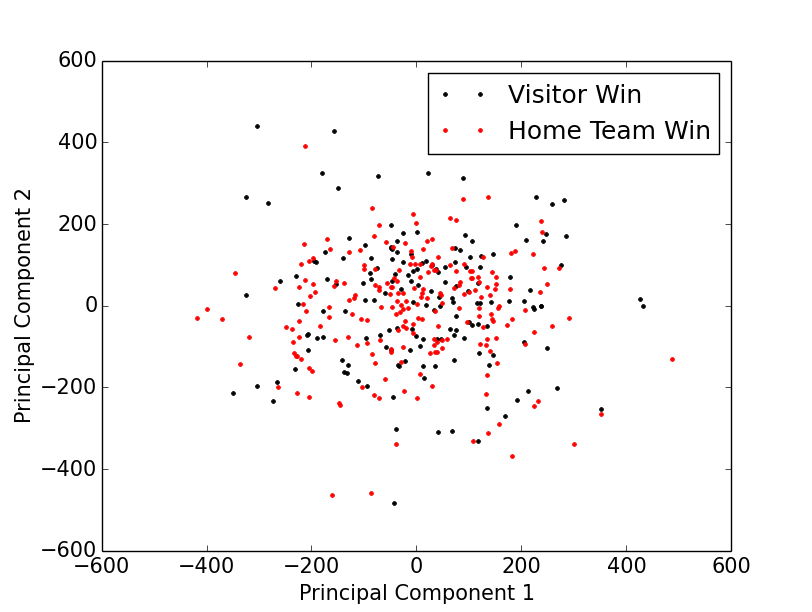
\includegraphics[scale=0.45]{figs/pca.png}
	\end{center}
	\caption{Game outcomes against the two most significant principal components of the feature data for prediction home team wins.}
	\label{fig::pca}
\end{figure}

\section{Model Development}
\subsection{Predicting Home Team Wins}
Several different models are developed using a variety of algorithms. These include decision trees with pruning, random forests, logistic regression, Naive Bayes, and Support Vector Machines (with both linear and Gaussian kernels). All of these models utilize validation data to tune hyper-parameters. For all models except the decision tree, the data is first transformed so that the training data has mean zero and standard deviation one for all features. This allows many of the algorithms to run more efficiently and converge to a reasonable solution. This transformation is not applied to the data given to decision trees since it should not make any difference. In the case of Support Vector Machines (SVM), the Gaussian kernel utilizes an L-2 regularization whereas the linear kernel uses an L-1 regularization to promote sparsity. The L-2 regularization is also applied for logistic regression.

The results of these models on the data are shown in Tab.~\ref{tab::try_1}. Notice that all models have similar misclassification errors of near 40\%. This error seems to be very high, but perhaps 60\% accuracy on game predictions is as good as we can expect. However, notice that some models have very high validation misclassification errors. Particularly, the random forest model has low training error (15\%) but  high validation error (43\%). The best model in terms of test error is the logistic regression model, but this model once again observes poor validation accuracy.

\begin{table}[ht!]
	\begin{center}
		\caption{Classification accuracy of several models applied to college football bowl data for predicting home team victories.}
		\label{tab::try_1}
		\begin{tabular}{l|ccc}
			\hline
			& \multicolumn{3}{c}{Misclassification Error} \\
			Model & Training & Validation & Test \\
			\hline
			Decision Tree w/ Pruning & 0.330 & 0.374 & 0.377\\
			Random Forest & 0.147 & 0.426 & 0.377\\
			Logistic Regression & 0.173 & 0.435 & 0.325\\
			Naive Bayes & 0.304 & 0.409 & 0.364\\
			SVM (Gaussian Kernel) & 0.304 & 0.383 & 0.390\\
			SVM (Linear Kernel) & 0.288 & 0.417 & 0.416\\
			\hline
		\end{tabular}
	\end{center}
\end{table}

The linear SVM model with L-1 regularization shows the worst test accuracy but does provide insight into the data through sparsity. After the tuned regularization penalty on validation data is applied, the linear SVM only uses 16 of the 97 available features. This motivates using only this reduced set of features in the other models. These 16 features are listed in Fig.~\ref{fig::reduced_features}. Of these 16 features, the line had by far the greatest weight.
\begin{figure}[ht!]
	\fbox{\parbox{\textwidth}{
	\begin{multicols}{3}
		\begin{itemize}
			\scriptsize
			\item Home Team Offensive Rush Yards
			\item Visitor Offensive Pass Yards
			\item Home Team Offensive Pass Yards vs. Bowl Teams
			\item Home Team Offensive Pass Attempts vs. Bowl Teams
			\item Home Team Defensive Pass Interceptions
			\item Home Team Defensive Rush Attempts
			\item Visitor Defensive Pass Interceptions
			\item Visitor Defensive Pass Completions
			\item Home Team Defensive Pass Interceptions vs. Bowl Teams
			\item Home Team Defensive Pass Completions vs. Bowl Teams
			\item Visitor Defensive Pass Interceptions vs. Bowl Teams
			\item Visitor Defensive Pass Completions vs. Bowl Teams
			\item Visitor Defensive Pass Yards vs. Bowl Teams
			\item Visitor Points Against vs. Bowl Teams
			\item Visitor Takeaways vs. Bowl Teams
			\item Line
		\end{itemize}
	\end{multicols}}}
	\caption{Features with nonzero coefficients in the linear SVM model with L-1 regularization.}
	\label{fig::reduced_features}
\end{figure}

All the models except the linear SVM model are trained on this reduced dataset. The results are shown in Table~\ref{tab::try_1_reduced}.
\begin{table}[ht!]
	\begin{center}
		\caption{Classification accuracy of several models applied to college football bowl data for predicting home team victories on a trimmed dataset.}
		\label{tab::try_1_reduced}
		\begin{tabular}{l|ccc}
			\hline
			& \multicolumn{3}{c}{Misclassification Error} \\
			Model & Training & Validation & Test \\
			\hline
			Decision Tree w/ Pruning & 0.330 & 0.374 & 0.377\\
			Random Forest & 0.073 & 0.426 & 0.364\\
			Logistic Regression & 0.283 & 0.452 & 0.351\\
			Naive Bayes & 0.267 & 0.417 & 0.299\\
			SVM (Gaussian Kernel) & 0.293 & 0.383 & 0.351\\
			\hline
		\end{tabular}
	\end{center}
\end{table}
With this reduced dataset we see an improvement in the random forest model, the Naive Bayes model, and the SVM with a Gaussian kernel. However, the logistic regression model increased its misclassification errors and the decision tree remained exactly the same. Digging further into the structure of the decision tree, we see that it is simply a decision stump based on the line, as shown in Fig.~\ref{fig::stump}.

\begin{figure}[h!]
	\begin{center}
		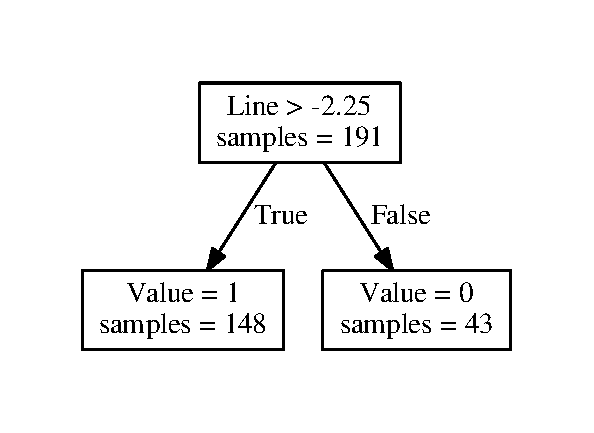
\includegraphics[scale=0.8]{figs/stump.pdf}
	\end{center}
	\caption{Decision stump formed from the decision tree algorithm.}
	\label{fig::stump}
\end{figure}

This result is quite unsatisfying since a model based purely on the Vegas betting line does not provide any interesting information. This indicates that any trends found further down the tree were pruned because they over-fitted the data and did not perform well in validation. The pruning is conducted by first fully forming the decision tree with no regularization penalty. Then a regularized error $\epsilon_R$ is calculated as
\begin{equation}
\epsilon_R = \sum_{i=1}^N |y_i - f(x_i)| + \alpha |T|
\end{equation}
where $\sum_{i=1}^N |y_i - f(x_i)|$ represents the training misclassification error and $|T|$ represents the number of leaves in the tree. The parameter $\alpha$ is determined from validation data yielding the smallest misclassification error. Starting at the leaves of the tree, decision nodes are turned into leaves if the regularized error does not increase with its removal. This result implies that only the decision based on the Vegas betting line generalized well. However, it is interesting to note that the decision boundary is not taken at zero. Intuitively, if a decision stump were created with the line it should be about zero (meaning even odds). This is a pure manifestation of statistical fluctuation in the training data. It seems that the partitioned training data has more home team wins than losses. Since bowl games are played on neutral fields, there should be no large preference for one side or the other. The home and away titles are nearly randomly assigned. 

\subsection{Predicting Upsets}
This motivates a re-casting of our problem. Instead of assigning labels based on whether the home team wins or loses, the problem is recast in terms of whether an upset occurs. More specifically, the label 0 is assigned to games in which the favored team wins and the label 1 is assigned to games in which the underdog wins. This requires a slight reworking of the features to be in terms of favored and underdog teams. In addition, the absolute value of the line is presented since the line is given in terms of how much the home team is favored. After taking the absolute value, it represents the general confidence that the favored team will win. A similar casting has been attempted by some in the past with limited success \cite{Padron}.

Despite the change of labels, many of the properties observed before are still true. For instance, the data is still highly mixed and no clear separation can be visible with respect to a few features by the human eye. This can be observed by again performing a principal component analysis and looking at how the labels correlated with the two largest principal components. This is shown in Fig.~\ref{fig::pca2} which shows little difference from the previous analysis shown in Fig.~\ref{fig::pca}.

\begin{figure}[h!]
	\begin{center}
		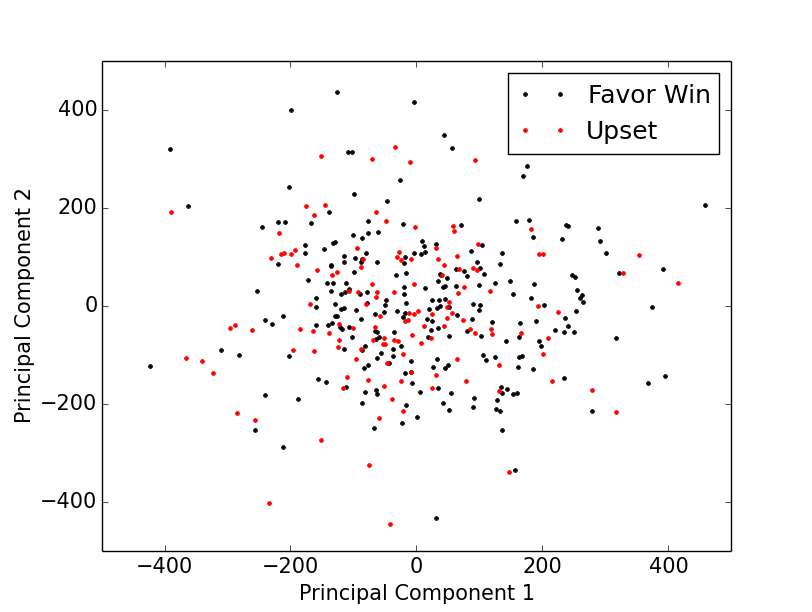
\includegraphics[scale=0.45]{figs/pca2.png}
	\end{center}
	\caption{Game outcomes against the two most significant principal components of the feature data for predicting upsets.}
	\label{fig::pca2}
\end{figure}

The results of the new formulation are presented in Table~\ref{tab::try_2} using the same train, validate, and test partitions as before.
\begin{table}[ht!]
	\begin{center}
		\caption{Classification accuracy of several models applied to college football bowl data for predicting bowl game upsets.}
		\label{tab::try_2}
		\begin{tabular}{l|ccc}
			\hline
			& \multicolumn{3}{c}{Misclassification Error} \\
			Model & Training & Validation & Test \\
			\hline
			Decision Tree w/ Pruning & 0.335 & 0.383 & 0.364\\
			Random Forest & 0.099 & 0.365 & 0.377\\
			Logistic Regression & 0.168 & 0.348 & 0.338\\
			Naive Bayes & 0.330 & 0.504 & 0.429\\
			SVM (Gaussian Kernel) & 0.283 & 0.330 & 0.364\\
			SVM (Linear Kernel) & 0.293 & 0.374 & 0.364\\
			\hline
		\end{tabular}
	\end{center}
\end{table}
We see that most models have comparable misclassification errors with the predictions based on the home team winning. However, for the best performing models such as SVM, logistic regression, and random forest, the validation errors and test errors are now both reasonably low. Naive Bayes seems to have great difficulty on this dataset. This is likely due to two factors. First, as we observed in section 3, some features have significantly non-normal distributions, violating the assumptions of Naive Bayes. Second, Naive Bayes does not have the same straightforward tuning parameters as other models so generalizing to new data can be difficult.

Just as before, we can use the nonzero weighted features from the linear SVM to form a trimmed dataset on which to train. This time, there are just 13 features and no single feature has incredibly high weight -- unlike our previous problem where the line received a very large weight. The features for the trimmed dataset are given in Figure~\ref{fig::trimmed_features}.
\begin{figure}[ht!]
	\fbox{\parbox{\textwidth}{
	\begin{multicols}{3}
		\begin{itemize}
			\scriptsize
			\item Favored Team Giveaways vs. Bowl Teams
			\item Favored Team Defensive Completions vs. Bowl Teams
			\item Favored Team Defensive Fumbles vs. Bowl Teams
			\item Underdog Defensive Pass Interceptions
			\item Underdog Defensive Pass Completions
			\item Underdog Offensive Rush Yards
			\item Underdog Average Points
			\item Underdog Average Points Against vs. Bowl Teams
			\item Underdog Losses vs. Bowl Teams
			\item Underdog Fumbles vs. Bowl Teams
			\item Underdog Defensive Pass Yards vs. Bowl Teams
			\item Difference in Offensive Pass Yards vs. Bowl Teams
			\item Magnitude of the Line
		\end{itemize}
	\end{multicols}}}
	\caption{Features with nonzero coefficients in the linear SVM model on upset predictions with L-1 regularization.}
	\label{fig::trimmed_features}
\end{figure}

Again, all models aside from the linear SVM model are re-trained on the reduced dataset. The results are displayed in Table~\ref{tab::try_2_reduced}. Notice that the reduced set helps the Random Forest model and the Naive Bayes model. This is probably because these two models do not have a regularization penalty as straightforward as SVMs and logistic regression which can directly penalize complexity. Therefore, the reduced complexity of the trimmed feature set aids those models.
\begin{table}[ht!]
	\begin{center}
		\caption{Classification accuracy of several models applied to college football bowl data for predicting upsets on a trimmed dataset.}
		\label{tab::try_2_reduced}
		\begin{tabular}{l|ccc}
			\hline
			& \multicolumn{3}{c}{Misclassification Error} \\
			Model & Training & Validation & Test \\
			\hline
			Decision Tree w/ Pruning & 0.335 & 0.383 & 0.364\\
			Random Forest & 0.251 & 0.383 & 0.338\\
			Logistic Regression & 0.298 & 0.409 & 0.416\\
			Naive Bayes & 0.309 & 0.435 & 0.416\\
			SVM (Gaussian Kernel) & 0.325 & 0.348 & 0.364\\
			\hline
		\end{tabular}
	\end{center}
\end{table}

Also, notice that the decision tree again is unchanged. Upon further investigation the pruned decision tree is less than a stump -- it is just a leaf. The decision tree always predicts that the favored team will win. This is again unsettling, but does provide a basis with which we can compare the effectiveness of the models. It is clear that for any model to be legitimate, it must be more accurate than the decision tree model. Therefore, we can disregard all models aside from the random forest on the trimmed dataset and all models aside from the logistic regression model on the full dataset.

If one model must be selected, it seems that the logistic regression model on the full data set would be preferred. It has low error on all train, validate, and test datasets and seems to be relatively robust. The classification matrix for this model on test data is presented in Table~\ref{tab::class_matrix}.

\begin{table}[ht!]
	\begin{center}
		\caption{Classification matrix based on test data for the logistic regression model in predicting upsets.}
		\label{tab::class_matrix}
		\begin{tabular}{l|cc}
			& \multicolumn{2}{c}{Actual} \\
			Predicted & Favored Team Wins & Upset \\
			\hline
			Favored Team Wins & 38 & 15\\
			Upset & 11 & 13\\
		\end{tabular}
	\end{center}
\end{table}

We see that the classification matrix seems to be relatively well behaved in the sense that we are making approximately equal type 1 and type 2 errors. Still, our accuracy is not as good as I had hoped entering this project. This has been observed in the past by other attempts \cite{Liu,Hamann} at predicting college football outcomes. One reason college football bowl games are particularly hard to predict is that competing teams are ideally chosen of similar strength. Therefore an advantage one team has in a few features might be compensated by a disadvantage in other features. Adding in large statistical noise associated with sports games, it can be particularly hard for algorithms to decipher trends. Even if the true underlying trends are recovered from the data, the statistical variation might be so large that misclassification error remains large.

Finally, with the logistic regression model chosen as the best model, we can use it to easily extract probabilities of upsets. This should give us information about the confidence level on each game. The strategy would be to pick the team with the highest probability of winning and then place the highest amount of points on the games 1 through $N$ where the probability of winning is the highest and place the lowest points on the games with lowest calculated winning probability. If we try this on our test set taking $N$ to be the number of data points in the test set (77), we calculate a \textbf{final score of 2043}.

This seems quite good as the highest number of possible points is 3003 so we are receiving 68\% of the possible point total. However, is this success due to the point placement strategy? To answer this question, we should test against a null distribution where point values are randomly assigned. Since we wish to test only the point placement strategy, we should hold the number of correct predictions constant. Through repeated trials, the point placements are randomly shuffled to form a distribution of point totals in which 49/77 games are correctly predicted, the accuracy of our logistic regression model. The resulting distribution is shown in Fig.~\ref{fig::bootstrap}. From this distribution we can see that our value is higher than the mean, which is 1989. However, we our point total is not very significant as 2043 lies within one standard deviation of the Gaussian distribution. Altogether, while our model performs better than average, it is difficult to prove that it is significantly better than simply betting with the Vegas line and randomly assigning confidence points.

\begin{figure}[h!]
	\begin{center}
		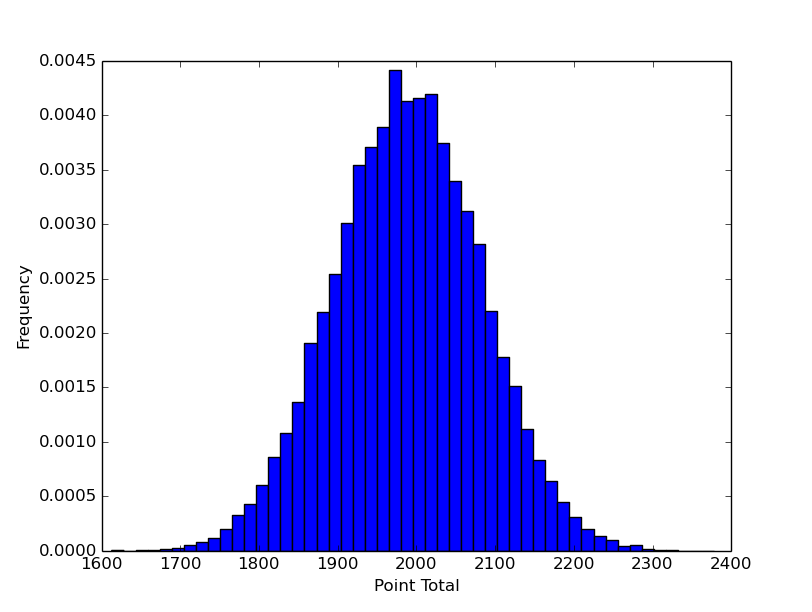
\includegraphics[scale=0.45]{figs/bootstrap_points.png}
	\end{center}
	\caption{Distribution of point totals by randomly selecting confidence points assignments assuming 49/77 games were correctly predicted.}
	\label{fig::bootstrap}
\end{figure}

\newpage
\section{Conclusion}

In this investigation, I attempted to form college football bowl predictions based on the statistics of the competing teams. This proved difficult as a clear separator in the data was not visible. The conditional distributions of the statistics for each class (wins and losses) largely overlapped. I tried re-casting the problem in terms of upset prediction which seemed a better posed problem. However, success was still marginal. The problem of predicting college football games is notoriously difficult due to the selection of teams to be evenly matched. Some of the final models developed did score higher than simply predicting the favored team, but the difference is not very significant. These models also allow for an estimation of the probabilities. Using these criteria, it is possible to form a ranking of the highest confidence games which resulted in a point total greater than that expected from a random assignment of confidence points. However, the difference once again is not very significant.

The models presented here could possibly be improved through the formation of better features. For instance, more intricate models for season performance could be determined based on the opponents. In the models developed here, a whole set of features is dedicated to performance against teams that finished their season with a bowl game. These features seem to be useful as many models prefer them over the season averaged features across all games. This could be taken a step further to include more comprehensive information regarding the team's opponents. There are a large number of other ways in which features could be added to the models to try to improve them, but the models and feature set presented here form a good starting point in which to understand the underlying behavior of college football bowl games.

\clearpage
\section*{Appendix A}
This appendix

\lstinputlisting[language=Python]{../data_extractor.py}

\clearpage
\bibliography{references}
\bibliographystyle{unsrt}

\end{document}